\documentclass[9pt, a4paper, twocolumn]{article}
% Packeges
\usepackage{fancyhdr}
\usepackage{graphicx}

% Fancy header package
\pagestyle{fancy}
\rhead{86411 - Filipe Marques - A097}
\lhead{IArt - Projeto 2}


% Title
\author{86411 - Filipe dos Santos Oliveira Marques}
\title{Projeto Inteligência Artificial(3º Ano , 1º Semestre 2018/2019)}

\begin{document}
\maketitle
% Parte 1 - Inferência Exata em Redes Bayesianas
\section{Parte 1}
\hspace{10mm}Nesta secção vamos analisar a solução produzida para a primeira parte do projeto - Inferência Exata em Redes Bayesianas.
\subsection{Análise dos Resultados}
\begin{figure}[h!]
	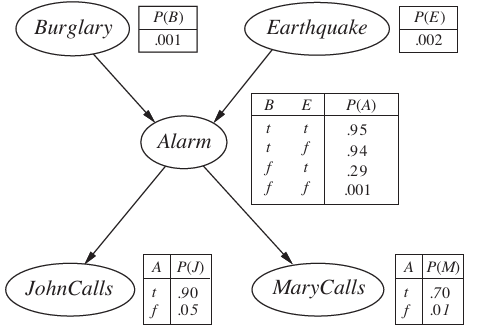
\includegraphics[scale=.45]{images/bn-b.png}
	\caption{Bayesian Network}
	\label{fig:bn1}
\end{figure}
A Figura \ref{fig:bn1} mostra a rede bayesiana utilizada para testar o algoritmos produzidos. \\
Os valores pedidos no enunciado foram todos calculados com sucesso e os resultados das \textit{queries} são:
\begin{itemize}
\item $P(B| j=t, m=t)=0.2842$
\item $P(E| j=t, m=t)=0.176$
\item $P(J| a=t, e=f)=0.900$
\end{itemize}
\subsection{Implementação}
\subsubsection{Probabilidade Conjunta}
\hspace{10mm}Para calcular a probabilidade conjunta temos de ter em conta algumas asserções em redes Bayesianas, nomeadamente que:
\begin{itemize}
\item Trata-se de uma rede acíclica; 
\item Cada nó é independente dos seus nós não descentes dado os seus predecessores imediatos(\textit{parents});
\end{itemize}
Sabendo isto, podemos definir a probabilidade conjunta:
\begin{center}
$P(y_{1},...,y_{n}) = \displaystyle\prod_{i=1}^{n}P(y_{i}|Parents(y_{i}))$ 
\end{center}
Onde $Y = \{y_{1},..., y_{n}\}$ representa o conjunto de variáveis na rede Bayesiana.
\begin{itemize}
\item \textbf{Desvantagens desta abordagem:}
\begin{itemize}
\item Tamanho das tabelas de probabilidade conjunta é exponencial \emph{$O(2^n)$}.
\end{itemize}
\end{itemize}
\subsubsection{Probabilidade Posterior}
\hspace{10mm}Para calcular a probabilidade posterior podes usar a probabilidade condicional. Por exemplo, para calcular a probabilidade de haver um \textit{Burglar} sabendo que \textit{JohnCalls} e \textit{MaryCalls} temos:
\begin{center}
$P(B|j=t, m=t)=\displaystyle\frac{P(B,j,m)}{P(j,m)}=\alpha P(B,j,m)$
\end{center}
Para calcular a probabilidade $P(B, j, m)$ temos somar as probabilidades conjuntas para todos os valores de '$e$' e '$a$' onde $j=t$ e $m=t$.\\
Assim:
\begin{center}
$P(B, j, m) = \displaystyle\sum_{e}\sum_{a}P(B, j, m, e, a)$
\end{center}
Tendo conhecimento da rede e das condições de independência podemos reescrever a segunda parte da equação como:
\begin{center}
$\displaystyle\sum_{e}\sum_{a}P(B)P(j|A)P(m|A)P(e)P(A|B,e)$
\end{center}
Agrupando os fatores temos que:
\begin{center}
$P(B)\displaystyle\sum_{e}P(e)\displaystyle\sum_{a}P(A|B, e)P(m|A)P(j|A)$
\end{center}
Esta abordagem de calcular a probabilidade posterior é chamada de enumeração. Para calcular a probabilidade posterior usamos o algoritmo \emph{Enumeration-Ask}.
\begin{itemize}
\item \textbf{Vantagens desta abordagem:}
\begin{itemize}
\item Permite reduzir o custo de calcular as probabilidades fase à abordagem da probabilidade conjunta.
\end{itemize}
\item \textbf{Limitações:}
\begin{itemize}
\item Esta abordagem não é ótima visto alguns valores serem calculados várias vezes ao longo da computação da probabilidade posterior.
\end{itemize}
\end{itemize}
\subsection{Complexidade Computacional}
\subsubsection{Probabilidade Conjunta}
Um nó $X_{i}$ com $k$ nós pais vai ter $2^k$ linhas na sua
tabela de probabilidade condicional.\\
\\
Cada linha vai guardar um valor $p$ para $X_{i}=t$. Assim para uma rede onde
 cada nó não tem mais de $k$ nós pais, vamos precisar de $O(n2^k)$ números.
Ao seja, cresce \textbf{\emph{linearmente}} com n (o número de nós na rede).
\subsubsection{Probabilidade Posterior}
Sabendo que a rede em estudo é \textit{\textbf{singly connected}}\footnote{Há no máximo uma ligação entre dois nós na rede.}, \textit{a complexidade espacial e temporal de inferência exata é linear com o tamanho da rede}.\footnote{AIMA, pag.528, cap.14.4.3.}\\\\
Uma possível alternativa a este método seria: \textit{Variable Elimination} que permitiria fazer os cálculos uma vez e guardar para usar mais tarde quando forem necessários, melhorando assim substancialmente o algoritmo de enumeração.

% Parte 2 - Aprendizagem por Reforço
\section{Parte 2}
\hspace{10mm}Nesta secção vamos analisar a solução produzida para a segunda parte do projeto - Aprendizagem por Reforço.
%TODO

\end{document}